\documentclass{article}

\usepackage[utf8]{inputenc}
\usepackage[a4paper, total={7.5in, 10in}]{geometry}
\usepackage{braket}
\usepackage{xcolor}
\usepackage{amsmath}
\usepackage{amssymb}
\usepackage{amsfonts}
\usepackage{graphicx}
\usepackage{svg}
\usepackage{float}
\usepackage{tikz}
\usetikzlibrary{patterns,shapes.arrows}

\usepackage[ruled,vlined]{algorithm2e}
\usepackage{multicol}
\usepackage[backend=biber,style=alphabetic,sorting=ynt]{biblatex}
\usepackage{xcolor}
\usepackage{pgfplots}
\DeclareUnicodeCharacter{2212}{−}
\usepgfplotslibrary{groupplots,dateplot}
\pgfplotsset{compat=newest}

\addbibresource{sample.bib} %Import the bibliography file

\newcommand{\commentt}[1]{\textcolor{blue}{ \textbf{[COMMENT]} #1}}
\newcommand{\ctt}[1]{\commentt{#1}}
\newcommand{\prb}[1]{ \mathbf{Pr} \left[ {#1} \right]}
\newcommand{\onotation}[1]{\(\mathcal{O} \left( {#1}  \right) \)}
\newcommand{\ona}[1]{\onotation{#1}}
\newcommand{\PSI}{{\ket{\psi}}}
\newcommand{\LESn}{\ket{\psi_n}}
\newcommand{\LESa}{\ket{\phi_n}}
\newcommand{\LESs}{\frac{1}{\sqrt{n}}\sum_{i}{\ket{\left(0^{i}10^{n-i}\right)^{n}}}}
\newcommand{\Hn}{\mathcal{H}_{n}}
\newcommand{\Ep}{\frac{1}{\sqrt{2^n}}\sum^{2^n}_{x}{ \ket{xx}}}
\newcommand{\HON}{\ket{\psi_{\text{honest}}}}
\newcommand{\Lemma}{\paragraph{Lemma.}}
\newcommand{\PonB}{ \rho + \frac{5}{16}\delta\le \frac{3}{4} + \frac{1}{16} } 
\newcommand{\Cpa}{[n, \rho n, \delta n]}
%\setlength{\columnsep}{0.6cm}

\newcommand{\Gz}{ G_{z}^{\delta} } 

\begin{document}


\title{Good Codes Singleton Bound}
\author{David Ponarovsky}
\maketitle
\abstract{ We propose a new asymptotic upper bound on the trade-off between the rate and the distance of good error correction codes. }
\begin{multicols*}{2}
  \section{Preambles}Coding theory has emerged by the need to transfer information in noisy communication channels. By embedding a message in higher dimension space, one can guarantee robustness against possible faults. The ratio of the original content length to the passed message length is the rate of the code, and it measures how consuming our communication protocol is. Furthermore, the distance of the code quantifies how many faults the scheme can absorb such that the receiver could recover the original message.    

  Even though it is obvious that any construction resilient to a large number of faults should have a complexity price, The exact relation between the rate and the code distance is still unknown. However, we do know un-tight upper bounds. The first one was proved by Singelton and set the linear constraint: $\rho + \delta \le 1 - \frac{1}{\Delta} $ for any $\left[ \Delta, \rho \Delta, \delta\Delta \right]$ linear code \cite{Singleton}.  

  Non-formally, we say that code is good if its distance and rate are scaled linearly in the encoded message length. Besides the fact that good codes are considered efficient in terms of robustness and overhead, they are also vital components in establishing secure multiparty computation \cite{MultiParty} and have a deep connection to probabilistic proofs.

In this work, we show a new upper bound $\PonB $ which tighter than the Singelton bound and holds for any Good code. First, we state the notations, definitions, and formal theorem in section 2. Then in sections 3 and 4, we review past results and provide their proofs in order to make this paper self-contained. Readers familiar with the basic concepts of LDPC codes and the Tanner code construction should consider skipping directly to section 5, in which we provide our proof. 
%Linear Error Correction Codes, 
\section{Notations, Definitions, And Our Contribution}
Here we focus only on linear binary codes, which one could think about as linear subspaces of $\mathbb{F}_{2}^{n}$. A common way to measure resilience is to ask how many bits an evil entity needs to flip such that the corrupted vector will be closer to another vector in that space than the original one. Those ideas were formulated by Hamming \cite{Hamming}, who presented the following definitions. 
\paragraph{Definition.} Let $n \in \mathbb{N}$ and $\rho, \delta\in \left( 0,1 \right)$. We say that $C$ is a \textit{binary linear code} with parameters $[n, \rho n, \delta n]$. If $C$ is a subspace of $\mathbb{F}_{2}^{n}$, and the dimension of $C$ is at least $\rho n$. In addition, we call the vectors belong to $C$ \textit{codewords} and define the distance of $C$ to be the minimal number of different bits between any codewords pair of $C$.   

From now on, we will use the term code to refer to linear binary codes, as we don't deal with any other types of codes. Also, even though it is customary to use the above parameters to analyze codes, we will use their percent forms called the relative distance and the rate of code, matching $\delta$ and $\rho$ correspondingly.     
\paragraph{Definition.} A \textit{family of codes} is an infinite series of codes. Additionally, suppose the rates and relative distances converge into constant values $\rho,\delta$. In that case, we abuse the notation and call that family of codes a code with $[n, \rho n, \delta n]$ for fixed $\rho, \delta\in [ 0,1 )$, and infinite integers $n \in \mathbb{N}$.     

Notice that the above definition contains codes with parameters attending to zero. From a practical view, it means that etiher we send too many bits, more than a constant amount, on each bit in the original message. Or that for big enough $n$, adversarial, limited to changing only a constant fraction of the bits, could disrupt the transmission. That distinction raises the definition of good codes.

\paragraph{Definition.}We will say that a family of codes is a \textit{good code} if its parameters converge into positive values. 


Nowadays, we are aware of a wide range of constructions yield good codes, including the expander codes of Sipser and Spilman \cite{ExpanderCodes} and the LTC codes of Dinur \cite{Dinur}, \cite{Pavel}, \cite{leverrier2022quantum}. Thus if, a decade ago, the main question was how to construct a good code, then now it is replaced by what is the best code one could expect.   

To get a feeling of the behavior of the distance-rate trade-of, Let us consider the following two codes; each demonstrates a different extreme case. First, define the repetition code $C_{r} \subset \mathbb{F}_{2}^{n \cdot r}$, In which, for a fixed integer $r$, any bit of the original string is duplicated $r$ times. Second, consider the parity check code $C_{p} \subset \mathbb{F}_{2}^{n+1}$, which it's codewords are only the vectors with even parity. Let us analyze the repetition code. Clearly, any two $n$-bits different messages must have at least a single different bit. Therefore their corresponding encoded codewords have to differ in at least $r$ bits. Hence, by scaling $r$, one could achieve a higher distance as he wishes. Sadly the rate of the code decays as $n/nr = 1/r$. In contrast, the parity check code adds only a single extra bit for the original message. Therefore scaling $n$ gives a family which has a rate attends to $\rho \rightarrow 1$. However, flipping any two different bits of a valid codeword is conversing the parity and, as a result, leads to another valid codeword.

To summarize the above, we have that, using a simple construction, one could construct the codes $[r, 1, r]$, $[r, r-1, 2]$. Each has a single perfect parameter while the other decays to the worst. In the next section, we will review the Singleton bound, which states that for any code (not necessarily good), there must be a zero-sum game between the relative distance and the rate.
Now, we are ready to formulate our contribution. 

\paragraph{Theorem 1}  Let $C$ be a family of good codes, with parameters $\Cpa$ . Then: \begin{equation*}
  \begin{split}
    & \PonB 
  \end{split}
\end{equation*}

\begin{figure}[H]
 % \centering
% This file was created with tikzplotlib v0.10.1.
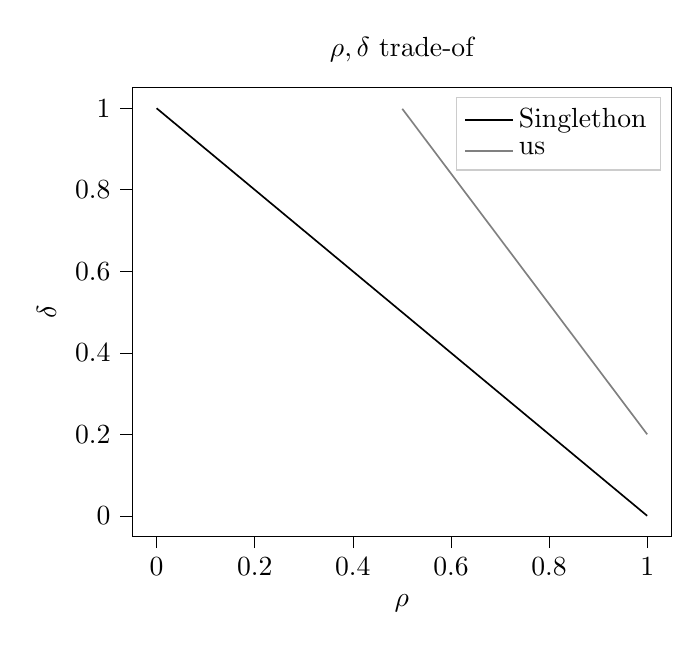
\begin{tikzpicture}

\definecolor{darkgray176}{RGB}{176,176,176}
\definecolor{gray}{RGB}{128,128,128}
\definecolor{lightgray204}{RGB}{204,204,204}

\begin{axis}[
legend cell align={left},
legend style={fill opacity=0.8, draw opacity=1, text opacity=1, draw=lightgray204},
tick align=outside,
tick pos=left,
title={\(\displaystyle  \rho,\delta\) trade-of },
x grid style={darkgray176},
xlabel={\(\displaystyle  \rho \) },
xmin=-0.05, xmax=1.05,
xtick style={color=black},
y grid style={darkgray176},
ylabel={\(\displaystyle  \delta \) },
ymin=-0.05, ymax=1.05,
ytick style={color=black}
]
\addplot [semithick, black]
table {%
0 1
0.00166944908180301 0.998330550918197
0.00333889816360601 0.996661101836394
0.00500834724540901 0.994991652754591
0.00667779632721202 0.993322203672788
0.00834724540901502 0.991652754590985
0.010016694490818 0.989983305509182
0.011686143572621 0.988313856427379
0.013355592654424 0.986644407345576
0.015025041736227 0.984974958263773
0.01669449081803 0.98330550918197
0.0183639398998331 0.981636060100167
0.0200333889816361 0.979966611018364
0.0217028380634391 0.978297161936561
0.0233722871452421 0.976627712854758
0.0250417362270451 0.974958263772955
0.0267111853088481 0.973288814691152
0.0283806343906511 0.971619365609349
0.0300500834724541 0.969949916527546
0.0317195325542571 0.968280467445743
0.0333889816360601 0.96661101836394
0.0350584307178631 0.964941569282137
0.0367278797996661 0.963272120200334
0.0383973288814691 0.961602671118531
0.0400667779632721 0.959933222036728
0.0417362270450751 0.958263772954925
0.0434056761268781 0.956594323873122
0.0450751252086811 0.954924874791319
0.0467445742904841 0.953255425709516
0.0484140233722871 0.951585976627713
0.0500834724540902 0.94991652754591
0.0517529215358932 0.948247078464107
0.0534223706176962 0.946577629382304
0.0550918196994992 0.944908180300501
0.0567612687813022 0.943238731218698
0.0584307178631052 0.941569282136895
0.0601001669449082 0.939899833055092
0.0617696160267112 0.938230383973289
0.0634390651085142 0.936560934891486
0.0651085141903172 0.934891485809683
0.0667779632721202 0.93322203672788
0.0684474123539232 0.931552587646077
0.0701168614357262 0.929883138564274
0.0717863105175292 0.928213689482471
0.0734557595993322 0.926544240400668
0.0751252086811352 0.924874791318865
0.0767946577629382 0.923205342237062
0.0784641068447412 0.921535893155259
0.0801335559265442 0.919866444073456
0.0818030050083473 0.918196994991653
0.0834724540901502 0.91652754590985
0.0851419031719533 0.914858096828047
0.0868113522537563 0.913188647746244
0.0884808013355593 0.911519198664441
0.0901502504173623 0.909849749582638
0.0918196994991653 0.908180300500835
0.0934891485809683 0.906510851419032
0.0951585976627713 0.904841402337229
0.0968280467445743 0.903171953255426
0.0984974958263773 0.901502504173623
0.10016694490818 0.89983305509182
0.101836393989983 0.898163606010017
0.103505843071786 0.896494156928214
0.105175292153589 0.894824707846411
0.106844741235392 0.893155258764608
0.108514190317195 0.891485809682805
0.110183639398998 0.889816360601002
0.111853088480801 0.888146911519199
0.113522537562604 0.886477462437396
0.115191986644407 0.884808013355593
0.11686143572621 0.88313856427379
0.118530884808013 0.881469115191987
0.120200333889816 0.879799666110184
0.121869782971619 0.878130217028381
0.123539232053422 0.876460767946578
0.125208681135225 0.874791318864775
0.126878130217028 0.873121869782972
0.128547579298831 0.871452420701169
0.130217028380634 0.869782971619366
0.131886477462437 0.868113522537563
0.13355592654424 0.86644407345576
0.135225375626043 0.864774624373957
0.136894824707846 0.863105175292154
0.138564273789649 0.861435726210351
0.140233722871452 0.859766277128548
0.141903171953255 0.858096828046745
0.143572621035058 0.856427378964942
0.145242070116861 0.854757929883139
0.146911519198664 0.853088480801336
0.148580968280467 0.851419031719532
0.15025041736227 0.849749582637729
0.151919866444073 0.848080133555926
0.153589315525876 0.846410684474123
0.155258764607679 0.84474123539232
0.156928213689482 0.843071786310517
0.158597662771285 0.841402337228714
0.160267111853088 0.839732888146911
0.161936560934891 0.838063439065108
0.163606010016695 0.836393989983305
0.165275459098498 0.834724540901502
0.1669449081803 0.8330550918197
0.168614357262103 0.831385642737897
0.170283806343907 0.829716193656094
0.17195325542571 0.828046744574291
0.173622704507513 0.826377295492488
0.175292153589316 0.824707846410685
0.176961602671119 0.823038397328882
0.178631051752922 0.821368948247079
0.180300500834725 0.819699499165276
0.181969949916528 0.818030050083473
0.183639398998331 0.816360601001669
0.185308848080134 0.814691151919866
0.186978297161937 0.813021702838063
0.18864774624374 0.81135225375626
0.190317195325543 0.809682804674457
0.191986644407346 0.808013355592654
0.193656093489149 0.806343906510851
0.195325542570952 0.804674457429048
0.196994991652755 0.803005008347245
0.198664440734558 0.801335559265442
0.200333889816361 0.799666110183639
0.202003338898164 0.797996661101836
0.203672787979967 0.796327212020033
0.20534223706177 0.79465776293823
0.207011686143573 0.792988313856427
0.208681135225376 0.791318864774624
0.210350584307179 0.789649415692821
0.212020033388982 0.787979966611018
0.213689482470785 0.786310517529215
0.215358931552588 0.784641068447412
0.217028380634391 0.782971619365609
0.218697829716194 0.781302170283806
0.220367278797997 0.779632721202003
0.2220367278798 0.7779632721202
0.223706176961603 0.776293823038397
0.225375626043406 0.774624373956594
0.227045075125209 0.772954924874791
0.228714524207012 0.771285475792988
0.230383973288815 0.769616026711185
0.232053422370618 0.767946577629382
0.233722871452421 0.766277128547579
0.235392320534224 0.764607679465776
0.237061769616027 0.762938230383973
0.23873121869783 0.76126878130217
0.240400667779633 0.759599332220367
0.242070116861436 0.757929883138564
0.243739565943239 0.756260434056761
0.245409015025042 0.754590984974958
0.247078464106845 0.752921535893155
0.248747913188648 0.751252086811352
0.250417362270451 0.749582637729549
0.252086811352254 0.747913188647746
0.253756260434057 0.746243739565943
0.25542570951586 0.74457429048414
0.257095158597663 0.742904841402337
0.258764607679466 0.741235392320534
0.260434056761269 0.739565943238731
0.262103505843072 0.737896494156928
0.263772954924875 0.736227045075125
0.265442404006678 0.734557595993322
0.267111853088481 0.732888146911519
0.268781302170284 0.731218697829716
0.270450751252087 0.729549248747913
0.27212020033389 0.72787979966611
0.273789649415693 0.726210350584307
0.275459098497496 0.724540901502504
0.277128547579299 0.722871452420701
0.278797996661102 0.721202003338898
0.280467445742905 0.719532554257095
0.282136894824708 0.717863105175292
0.283806343906511 0.716193656093489
0.285475792988314 0.714524207011686
0.287145242070117 0.712854757929883
0.28881469115192 0.71118530884808
0.290484140233723 0.709515859766277
0.292153589315526 0.707846410684474
0.293823038397329 0.706176961602671
0.295492487479132 0.704507512520868
0.297161936560935 0.702838063439065
0.298831385642738 0.701168614357262
0.300500834724541 0.699499165275459
0.302170283806344 0.697829716193656
0.303839732888147 0.696160267111853
0.30550918196995 0.69449081803005
0.307178631051753 0.692821368948247
0.308848080133556 0.691151919866444
0.310517529215359 0.689482470784641
0.312186978297162 0.687813021702838
0.313856427378965 0.686143572621035
0.315525876460768 0.684474123539232
0.317195325542571 0.682804674457429
0.318864774624374 0.681135225375626
0.320534223706177 0.679465776293823
0.32220367278798 0.67779632721202
0.323873121869783 0.676126878130217
0.325542570951586 0.674457429048414
0.327212020033389 0.672787979966611
0.328881469115192 0.671118530884808
0.330550918196995 0.669449081803005
0.332220367278798 0.667779632721202
0.333889816360601 0.666110183639399
0.335559265442404 0.664440734557596
0.337228714524207 0.662771285475793
0.33889816360601 0.66110183639399
0.340567612687813 0.659432387312187
0.342237061769616 0.657762938230384
0.343906510851419 0.656093489148581
0.345575959933222 0.654424040066778
0.347245409015025 0.652754590984975
0.348914858096828 0.651085141903172
0.350584307178631 0.649415692821369
0.352253756260434 0.647746243739566
0.353923205342237 0.646076794657763
0.35559265442404 0.64440734557596
0.357262103505843 0.642737896494157
0.358931552587646 0.641068447412354
0.360601001669449 0.639398998330551
0.362270450751252 0.637729549248748
0.363939899833055 0.636060100166945
0.365609348914858 0.634390651085142
0.367278797996661 0.632721202003339
0.368948247078464 0.631051752921536
0.370617696160267 0.629382303839733
0.37228714524207 0.62771285475793
0.373956594323873 0.626043405676127
0.375626043405676 0.624373956594324
0.377295492487479 0.622704507512521
0.378964941569282 0.621035058430718
0.380634390651085 0.619365609348915
0.382303839732888 0.617696160267112
0.383973288814691 0.616026711185309
0.385642737896494 0.614357262103506
0.387312186978297 0.612687813021703
0.3889816360601 0.6110183639399
0.390651085141903 0.609348914858097
0.392320534223706 0.607679465776294
0.393989983305509 0.606010016694491
0.395659432387312 0.604340567612688
0.397328881469115 0.602671118530885
0.398998330550918 0.601001669449082
0.400667779632721 0.599332220367279
0.402337228714524 0.597662771285476
0.404006677796327 0.595993322203673
0.40567612687813 0.59432387312187
0.407345575959933 0.592654424040067
0.409015025041736 0.590984974958264
0.410684474123539 0.589315525876461
0.412353923205342 0.587646076794658
0.414023372287145 0.585976627712855
0.415692821368948 0.584307178631052
0.417362270450751 0.582637729549249
0.419031719532554 0.580968280467446
0.420701168614357 0.579298831385643
0.42237061769616 0.57762938230384
0.424040066777963 0.575959933222037
0.425709515859766 0.574290484140234
0.427378964941569 0.572621035058431
0.429048414023372 0.570951585976628
0.430717863105175 0.569282136894825
0.432387312186978 0.567612687813022
0.434056761268781 0.565943238731219
0.435726210350584 0.564273789649416
0.437395659432387 0.562604340567613
0.43906510851419 0.56093489148581
0.440734557595993 0.559265442404007
0.442404006677796 0.557595993322204
0.444073455759599 0.555926544240401
0.445742904841402 0.554257095158598
0.447412353923205 0.552587646076795
0.449081803005008 0.550918196994992
0.450751252086811 0.549248747913189
0.452420701168614 0.547579298831386
0.454090150250417 0.545909849749583
0.45575959933222 0.54424040066778
0.457429048414023 0.542570951585977
0.459098497495826 0.540901502504174
0.460767946577629 0.539232053422371
0.462437395659432 0.537562604340568
0.464106844741235 0.535893155258765
0.465776293823038 0.534223706176962
0.467445742904841 0.532554257095159
0.469115191986644 0.530884808013356
0.470784641068447 0.529215358931553
0.47245409015025 0.52754590984975
0.474123539232053 0.525876460767947
0.475792988313856 0.524207011686143
0.477462437395659 0.52253756260434
0.479131886477462 0.520868113522537
0.480801335559265 0.519198664440734
0.482470784641068 0.517529215358931
0.484140233722871 0.515859766277128
0.485809682804674 0.514190317195325
0.487479131886477 0.512520868113522
0.48914858096828 0.510851419031719
0.490818030050084 0.509181969949916
0.492487479131887 0.507512520868113
0.49415692821369 0.50584307178631
0.495826377295493 0.504173622704507
0.497495826377296 0.502504173622704
0.499165275459099 0.500834724540901
0.500834724540901 0.499165275459099
0.502504173622704 0.497495826377296
0.504173622704507 0.495826377295493
0.50584307178631 0.49415692821369
0.507512520868113 0.492487479131887
0.509181969949916 0.490818030050084
0.51085141903172 0.48914858096828
0.512520868113523 0.487479131886477
0.514190317195326 0.485809682804674
0.515859766277129 0.484140233722871
0.517529215358932 0.482470784641068
0.519198664440735 0.480801335559265
0.520868113522538 0.479131886477462
0.522537562604341 0.477462437395659
0.524207011686144 0.475792988313856
0.525876460767947 0.474123539232053
0.52754590984975 0.47245409015025
0.529215358931553 0.470784641068447
0.530884808013356 0.469115191986644
0.532554257095159 0.467445742904841
0.534223706176962 0.465776293823038
0.535893155258765 0.464106844741235
0.537562604340568 0.462437395659432
0.539232053422371 0.460767946577629
0.540901502504174 0.459098497495826
0.542570951585977 0.457429048414023
0.54424040066778 0.45575959933222
0.545909849749583 0.454090150250417
0.547579298831386 0.452420701168614
0.549248747913189 0.450751252086811
0.550918196994992 0.449081803005008
0.552587646076795 0.447412353923205
0.554257095158598 0.445742904841402
0.555926544240401 0.444073455759599
0.557595993322204 0.442404006677796
0.559265442404007 0.440734557595993
0.56093489148581 0.43906510851419
0.562604340567613 0.437395659432387
0.564273789649416 0.435726210350584
0.565943238731219 0.434056761268781
0.567612687813022 0.432387312186978
0.569282136894825 0.430717863105175
0.570951585976628 0.429048414023372
0.572621035058431 0.427378964941569
0.574290484140234 0.425709515859766
0.575959933222037 0.424040066777963
0.57762938230384 0.42237061769616
0.579298831385643 0.420701168614357
0.580968280467446 0.419031719532554
0.582637729549249 0.417362270450751
0.584307178631052 0.415692821368948
0.585976627712855 0.414023372287145
0.587646076794658 0.412353923205342
0.589315525876461 0.410684474123539
0.590984974958264 0.409015025041736
0.592654424040067 0.407345575959933
0.59432387312187 0.40567612687813
0.595993322203673 0.404006677796327
0.597662771285476 0.402337228714524
0.599332220367279 0.400667779632721
0.601001669449082 0.398998330550918
0.602671118530885 0.397328881469115
0.604340567612688 0.395659432387312
0.606010016694491 0.393989983305509
0.607679465776294 0.392320534223706
0.609348914858097 0.390651085141903
0.6110183639399 0.3889816360601
0.612687813021703 0.387312186978297
0.614357262103506 0.385642737896494
0.616026711185309 0.383973288814691
0.617696160267112 0.382303839732888
0.619365609348915 0.380634390651085
0.621035058430718 0.378964941569282
0.622704507512521 0.377295492487479
0.624373956594324 0.375626043405676
0.626043405676127 0.373956594323873
0.62771285475793 0.37228714524207
0.629382303839733 0.370617696160267
0.631051752921536 0.368948247078464
0.632721202003339 0.367278797996661
0.634390651085142 0.365609348914858
0.636060100166945 0.363939899833055
0.637729549248748 0.362270450751252
0.639398998330551 0.360601001669449
0.641068447412354 0.358931552587646
0.642737896494157 0.357262103505843
0.64440734557596 0.35559265442404
0.646076794657763 0.353923205342237
0.647746243739566 0.352253756260434
0.649415692821369 0.350584307178631
0.651085141903172 0.348914858096828
0.652754590984975 0.347245409015025
0.654424040066778 0.345575959933222
0.656093489148581 0.343906510851419
0.657762938230384 0.342237061769616
0.659432387312187 0.340567612687813
0.66110183639399 0.33889816360601
0.662771285475793 0.337228714524207
0.664440734557596 0.335559265442404
0.666110183639399 0.333889816360601
0.667779632721202 0.332220367278798
0.669449081803005 0.330550918196995
0.671118530884808 0.328881469115192
0.672787979966611 0.327212020033389
0.674457429048414 0.325542570951586
0.676126878130217 0.323873121869783
0.67779632721202 0.32220367278798
0.679465776293823 0.320534223706177
0.681135225375626 0.318864774624374
0.682804674457429 0.317195325542571
0.684474123539232 0.315525876460768
0.686143572621035 0.313856427378965
0.687813021702838 0.312186978297162
0.689482470784641 0.310517529215359
0.691151919866444 0.308848080133556
0.692821368948247 0.307178631051753
0.69449081803005 0.30550918196995
0.696160267111853 0.303839732888147
0.697829716193656 0.302170283806344
0.699499165275459 0.300500834724541
0.701168614357262 0.298831385642738
0.702838063439065 0.297161936560935
0.704507512520868 0.295492487479132
0.706176961602671 0.293823038397329
0.707846410684474 0.292153589315526
0.709515859766277 0.290484140233723
0.71118530884808 0.28881469115192
0.712854757929883 0.287145242070117
0.714524207011686 0.285475792988314
0.716193656093489 0.283806343906511
0.717863105175292 0.282136894824708
0.719532554257095 0.280467445742905
0.721202003338898 0.278797996661102
0.722871452420701 0.277128547579299
0.724540901502504 0.275459098497496
0.726210350584307 0.273789649415693
0.72787979966611 0.27212020033389
0.729549248747913 0.270450751252087
0.731218697829716 0.268781302170284
0.732888146911519 0.267111853088481
0.734557595993322 0.265442404006678
0.736227045075125 0.263772954924875
0.737896494156928 0.262103505843072
0.739565943238731 0.260434056761269
0.741235392320534 0.258764607679466
0.742904841402337 0.257095158597663
0.74457429048414 0.25542570951586
0.746243739565943 0.253756260434057
0.747913188647746 0.252086811352254
0.749582637729549 0.250417362270451
0.751252086811352 0.248747913188648
0.752921535893155 0.247078464106845
0.754590984974958 0.245409015025042
0.756260434056761 0.243739565943239
0.757929883138564 0.242070116861436
0.759599332220367 0.240400667779633
0.76126878130217 0.23873121869783
0.762938230383973 0.237061769616027
0.764607679465776 0.235392320534224
0.766277128547579 0.233722871452421
0.767946577629382 0.232053422370618
0.769616026711185 0.230383973288815
0.771285475792988 0.228714524207012
0.772954924874791 0.227045075125209
0.774624373956594 0.225375626043406
0.776293823038397 0.223706176961603
0.7779632721202 0.2220367278798
0.779632721202003 0.220367278797997
0.781302170283806 0.218697829716194
0.782971619365609 0.217028380634391
0.784641068447412 0.215358931552588
0.786310517529215 0.213689482470785
0.787979966611018 0.212020033388982
0.789649415692821 0.210350584307179
0.791318864774624 0.208681135225376
0.792988313856427 0.207011686143573
0.79465776293823 0.20534223706177
0.796327212020033 0.203672787979967
0.797996661101836 0.202003338898164
0.799666110183639 0.200333889816361
0.801335559265442 0.198664440734558
0.803005008347245 0.196994991652755
0.804674457429048 0.195325542570952
0.806343906510851 0.193656093489149
0.808013355592654 0.191986644407346
0.809682804674457 0.190317195325543
0.81135225375626 0.18864774624374
0.813021702838063 0.186978297161937
0.814691151919867 0.185308848080133
0.81636060100167 0.18363939899833
0.818030050083473 0.181969949916527
0.819699499165276 0.180300500834724
0.821368948247079 0.178631051752921
0.823038397328882 0.176961602671118
0.824707846410685 0.175292153589315
0.826377295492488 0.173622704507512
0.828046744574291 0.171953255425709
0.829716193656094 0.170283806343906
0.831385642737897 0.168614357262103
0.8330550918197 0.1669449081803
0.834724540901502 0.165275459098498
0.836393989983305 0.163606010016695
0.838063439065108 0.161936560934892
0.839732888146911 0.160267111853089
0.841402337228715 0.158597662771285
0.843071786310518 0.156928213689482
0.844741235392321 0.155258764607679
0.846410684474124 0.153589315525876
0.848080133555927 0.151919866444073
0.84974958263773 0.15025041736227
0.851419031719533 0.148580968280467
0.853088480801336 0.146911519198664
0.854757929883139 0.145242070116861
0.856427378964942 0.143572621035058
0.858096828046745 0.141903171953255
0.859766277128548 0.140233722871452
0.861435726210351 0.138564273789649
0.863105175292154 0.136894824707846
0.864774624373957 0.135225375626043
0.86644407345576 0.13355592654424
0.868113522537563 0.131886477462437
0.869782971619366 0.130217028380634
0.871452420701169 0.128547579298831
0.873121869782972 0.126878130217028
0.874791318864775 0.125208681135225
0.876460767946578 0.123539232053422
0.878130217028381 0.121869782971619
0.879799666110184 0.120200333889816
0.881469115191987 0.118530884808013
0.88313856427379 0.11686143572621
0.884808013355593 0.115191986644407
0.886477462437396 0.113522537562604
0.888146911519199 0.111853088480801
0.889816360601002 0.110183639398998
0.891485809682805 0.108514190317195
0.893155258764608 0.106844741235392
0.894824707846411 0.105175292153589
0.896494156928214 0.103505843071786
0.898163606010017 0.101836393989983
0.89983305509182 0.10016694490818
0.901502504173623 0.0984974958263772
0.903171953255426 0.0968280467445742
0.904841402337229 0.0951585976627712
0.906510851419032 0.0934891485809682
0.908180300500835 0.0918196994991652
0.909849749582638 0.0901502504173622
0.911519198664441 0.0884808013355592
0.913188647746244 0.0868113522537562
0.914858096828047 0.0851419031719532
0.91652754590985 0.0834724540901502
0.918196994991653 0.0818030050083473
0.919866444073456 0.0801335559265443
0.921535893155259 0.0784641068447413
0.923205342237062 0.0767946577629383
0.924874791318865 0.0751252086811351
0.926544240400668 0.0734557595993321
0.928213689482471 0.0717863105175292
0.929883138564274 0.0701168614357262
0.931552587646077 0.0684474123539232
0.93322203672788 0.0667779632721202
0.934891485809683 0.0651085141903172
0.936560934891486 0.0634390651085142
0.938230383973289 0.0617696160267112
0.939899833055092 0.0601001669449082
0.941569282136895 0.0584307178631052
0.943238731218698 0.0567612687813022
0.944908180300501 0.0550918196994992
0.946577629382304 0.0534223706176962
0.948247078464107 0.0517529215358932
0.94991652754591 0.0500834724540902
0.951585976627713 0.0484140233722871
0.953255425709516 0.0467445742904841
0.954924874791319 0.0450751252086811
0.956594323873122 0.0434056761268781
0.958263772954925 0.0417362270450751
0.959933222036728 0.0400667779632721
0.961602671118531 0.0383973288814691
0.963272120200334 0.0367278797996661
0.964941569282137 0.0350584307178631
0.96661101836394 0.0333889816360601
0.968280467445743 0.0317195325542571
0.969949916527546 0.0300500834724541
0.971619365609349 0.0283806343906511
0.973288814691152 0.0267111853088481
0.974958263772955 0.0250417362270451
0.976627712854758 0.0233722871452421
0.978297161936561 0.0217028380634391
0.979966611018364 0.020033388981636
0.981636060100167 0.018363939899833
0.98330550918197 0.01669449081803
0.984974958263773 0.015025041736227
0.986644407345576 0.013355592654424
0.988313856427379 0.011686143572621
0.989983305509182 0.010016694490818
0.991652754590985 0.00834724540901499
0.993322203672788 0.00667779632721199
0.994991652754591 0.005008347245409
0.996661101836394 0.003338898163606
0.998330550918197 0.001669449081803
1 0
};
\addlegendentry{Singlethon}
\addplot [semithick, gray]
table {%
0.500834724540901 0.998664440734558
0.502504173622704 0.995993322203673
0.504173622704507 0.993322203672788
0.50584307178631 0.990651085141903
0.507512520868113 0.987979966611019
0.509181969949916 0.985308848080134
0.51085141903172 0.982637729549249
0.512520868113523 0.979966611018364
0.514190317195326 0.977295492487479
0.515859766277129 0.974624373956594
0.517529215358932 0.97195325542571
0.519198664440735 0.969282136894825
0.520868113522538 0.96661101836394
0.522537562604341 0.963939899833055
0.524207011686144 0.96126878130217
0.525876460767947 0.958597662771286
0.52754590984975 0.955926544240401
0.529215358931553 0.953255425709516
0.530884808013356 0.950584307178631
0.532554257095159 0.947913188647746
0.534223706176962 0.945242070116862
0.535893155258765 0.942570951585977
0.537562604340568 0.939899833055092
0.539232053422371 0.937228714524207
0.540901502504174 0.934557595993322
0.542570951585977 0.931886477462437
0.54424040066778 0.929215358931553
0.545909849749583 0.926544240400668
0.547579298831386 0.923873121869783
0.549248747913189 0.921202003338898
0.550918196994992 0.918530884808013
0.552587646076795 0.915859766277129
0.554257095158598 0.913188647746244
0.555926544240401 0.910517529215359
0.557595993322204 0.907846410684474
0.559265442404007 0.905175292153589
0.56093489148581 0.902504173622705
0.562604340567613 0.89983305509182
0.564273789649416 0.897161936560935
0.565943238731219 0.89449081803005
0.567612687813022 0.891819699499165
0.569282136894825 0.88914858096828
0.570951585976628 0.886477462437396
0.572621035058431 0.883806343906511
0.574290484140234 0.881135225375626
0.575959933222037 0.878464106844741
0.57762938230384 0.875792988313856
0.579298831385643 0.873121869782972
0.580968280467446 0.870450751252087
0.582637729549249 0.867779632721202
0.584307178631052 0.865108514190317
0.585976627712855 0.862437395659432
0.587646076794658 0.859766277128548
0.589315525876461 0.857095158597663
0.590984974958264 0.854424040066778
0.592654424040067 0.851752921535893
0.59432387312187 0.849081803005008
0.595993322203673 0.846410684474123
0.597662771285476 0.843739565943239
0.599332220367279 0.841068447412354
0.601001669449082 0.838397328881469
0.602671118530885 0.835726210350584
0.604340567612688 0.8330550918197
0.606010016694491 0.830383973288815
0.607679465776294 0.82771285475793
0.609348914858097 0.825041736227045
0.6110183639399 0.82237061769616
0.612687813021703 0.819699499165276
0.614357262103506 0.817028380634391
0.616026711185309 0.814357262103506
0.617696160267112 0.811686143572621
0.619365609348915 0.809015025041736
0.621035058430718 0.806343906510851
0.622704507512521 0.803672787979967
0.624373956594324 0.801001669449082
0.626043405676127 0.798330550918197
0.62771285475793 0.795659432387312
0.629382303839733 0.792988313856427
0.631051752921536 0.790317195325543
0.632721202003339 0.787646076794658
0.634390651085142 0.784974958263773
0.636060100166945 0.782303839732888
0.637729549248748 0.779632721202003
0.639398998330551 0.776961602671119
0.641068447412354 0.774290484140234
0.642737896494157 0.771619365609349
0.64440734557596 0.768948247078464
0.646076794657763 0.766277128547579
0.647746243739566 0.763606010016695
0.649415692821369 0.76093489148581
0.651085141903172 0.758263772954925
0.652754590984975 0.75559265442404
0.654424040066778 0.752921535893155
0.656093489148581 0.75025041736227
0.657762938230384 0.747579298831386
0.659432387312187 0.744908180300501
0.66110183639399 0.742237061769616
0.662771285475793 0.739565943238731
0.664440734557596 0.736894824707846
0.666110183639399 0.734223706176962
0.667779632721202 0.731552587646077
0.669449081803005 0.728881469115192
0.671118530884808 0.726210350584307
0.672787979966611 0.723539232053422
0.674457429048414 0.720868113522538
0.676126878130217 0.718196994991653
0.67779632721202 0.715525876460768
0.679465776293823 0.712854757929883
0.681135225375626 0.710183639398998
0.682804674457429 0.707512520868113
0.684474123539232 0.704841402337229
0.686143572621035 0.702170283806344
0.687813021702838 0.699499165275459
0.689482470784641 0.696828046744574
0.691151919866444 0.694156928213689
0.692821368948247 0.691485809682805
0.69449081803005 0.68881469115192
0.696160267111853 0.686143572621035
0.697829716193656 0.68347245409015
0.699499165275459 0.680801335559265
0.701168614357262 0.678130217028381
0.702838063439065 0.675459098497496
0.704507512520868 0.672787979966611
0.706176961602671 0.670116861435726
0.707846410684474 0.667445742904841
0.709515859766277 0.664774624373957
0.71118530884808 0.662103505843072
0.712854757929883 0.659432387312187
0.714524207011686 0.656761268781302
0.716193656093489 0.654090150250417
0.717863105175292 0.651419031719533
0.719532554257095 0.648747913188648
0.721202003338898 0.646076794657763
0.722871452420701 0.643405676126878
0.724540901502504 0.640734557595993
0.726210350584307 0.638063439065109
0.72787979966611 0.635392320534224
0.729549248747913 0.632721202003339
0.731218697829716 0.630050083472454
0.732888146911519 0.627378964941569
0.734557595993322 0.624707846410684
0.736227045075125 0.6220367278798
0.737896494156928 0.619365609348915
0.739565943238731 0.61669449081803
0.741235392320534 0.614023372287145
0.742904841402337 0.61135225375626
0.74457429048414 0.608681135225376
0.746243739565943 0.606010016694491
0.747913188647746 0.603338898163606
0.749582637729549 0.600667779632721
0.751252086811352 0.597996661101836
0.752921535893155 0.595325542570952
0.754590984974958 0.592654424040067
0.756260434056761 0.589983305509182
0.757929883138564 0.587312186978297
0.759599332220367 0.584641068447412
0.76126878130217 0.581969949916528
0.762938230383973 0.579298831385643
0.764607679465776 0.576627712854758
0.766277128547579 0.573956594323873
0.767946577629382 0.571285475792988
0.769616026711185 0.568614357262104
0.771285475792988 0.565943238731219
0.772954924874791 0.563272120200334
0.774624373956594 0.560601001669449
0.776293823038397 0.557929883138564
0.7779632721202 0.55525876460768
0.779632721202003 0.552587646076795
0.781302170283806 0.54991652754591
0.782971619365609 0.547245409015025
0.784641068447412 0.54457429048414
0.786310517529215 0.541903171953255
0.787979966611018 0.539232053422371
0.789649415692821 0.536560934891486
0.791318864774624 0.533889816360601
0.792988313856427 0.531218697829716
0.79465776293823 0.528547579298831
0.796327212020033 0.525876460767947
0.797996661101836 0.523205342237062
0.799666110183639 0.520534223706177
0.801335559265442 0.517863105175292
0.803005008347245 0.515191986644407
0.804674457429048 0.512520868113523
0.806343906510851 0.509849749582638
0.808013355592654 0.507178631051753
0.809682804674457 0.504507512520868
0.81135225375626 0.501836393989983
0.813021702838063 0.499165275459099
0.814691151919867 0.496494156928214
0.81636060100167 0.493823038397329
0.818030050083473 0.491151919866444
0.819699499165276 0.488480801335559
0.821368948247079 0.485809682804674
0.823038397328882 0.48313856427379
0.824707846410685 0.480467445742905
0.826377295492488 0.47779632721202
0.828046744574291 0.475125208681135
0.829716193656094 0.47245409015025
0.831385642737897 0.469782971619366
0.8330550918197 0.467111853088481
0.834724540901502 0.464440734557596
0.836393989983305 0.461769616026711
0.838063439065108 0.459098497495826
0.839732888146911 0.456427378964942
0.841402337228715 0.453756260434057
0.843071786310518 0.451085141903172
0.844741235392321 0.448414023372287
0.846410684474124 0.445742904841402
0.848080133555927 0.443071786310517
0.84974958263773 0.440400667779633
0.851419031719533 0.437729549248748
0.853088480801336 0.435058430717863
0.854757929883139 0.432387312186978
0.856427378964942 0.429716193656093
0.858096828046745 0.427045075125209
0.859766277128548 0.424373956594324
0.861435726210351 0.421702838063439
0.863105175292154 0.419031719532554
0.864774624373957 0.416360601001669
0.86644407345576 0.413689482470785
0.868113522537563 0.4110183639399
0.869782971619366 0.408347245409015
0.871452420701169 0.40567612687813
0.873121869782972 0.403005008347245
0.874791318864775 0.400333889816361
0.876460767946578 0.397662771285476
0.878130217028381 0.394991652754591
0.879799666110184 0.392320534223706
0.881469115191987 0.389649415692821
0.88313856427379 0.386978297161937
0.884808013355593 0.384307178631052
0.886477462437396 0.381636060100167
0.888146911519199 0.378964941569282
0.889816360601002 0.376293823038397
0.891485809682805 0.373622704507513
0.893155258764608 0.370951585976628
0.894824707846411 0.368280467445743
0.896494156928214 0.365609348914858
0.898163606010017 0.362938230383973
0.89983305509182 0.360267111853088
0.901502504173623 0.357595993322204
0.903171953255426 0.354924874791319
0.904841402337229 0.352253756260434
0.906510851419032 0.349582637729549
0.908180300500835 0.346911519198664
0.909849749582638 0.34424040066778
0.911519198664441 0.341569282136895
0.913188647746244 0.33889816360601
0.914858096828047 0.336227045075125
0.91652754590985 0.33355592654424
0.918196994991653 0.330884808013356
0.919866444073456 0.328213689482471
0.921535893155259 0.325542570951586
0.923205342237062 0.322871452420701
0.924874791318865 0.320200333889816
0.926544240400668 0.317529215358931
0.928213689482471 0.314858096828047
0.929883138564274 0.312186978297162
0.931552587646077 0.309515859766277
0.93322203672788 0.306844741235392
0.934891485809683 0.304173622704507
0.936560934891486 0.301502504173623
0.938230383973289 0.298831385642738
0.939899833055092 0.296160267111853
0.941569282136895 0.293489148580968
0.943238731218698 0.290818030050083
0.944908180300501 0.288146911519199
0.946577629382304 0.285475792988314
0.948247078464107 0.282804674457429
0.94991652754591 0.280133555926544
0.951585976627713 0.277462437395659
0.953255425709516 0.274791318864775
0.954924874791319 0.27212020033389
0.956594323873122 0.269449081803005
0.958263772954925 0.26677796327212
0.959933222036728 0.264106844741235
0.961602671118531 0.261435726210351
0.963272120200334 0.258764607679466
0.964941569282137 0.256093489148581
0.96661101836394 0.253422370617696
0.968280467445743 0.250751252086811
0.969949916527546 0.248080133555927
0.971619365609349 0.245409015025042
0.973288814691152 0.242737896494157
0.974958263772955 0.240066777963272
0.976627712854758 0.237395659432387
0.978297161936561 0.234724540901503
0.979966611018364 0.232053422370618
0.981636060100167 0.229382303839733
0.98330550918197 0.226711185308848
0.984974958263773 0.224040066777963
0.986644407345576 0.221368948247078
0.988313856427379 0.218697829716194
0.989983305509182 0.216026711185309
0.991652754590985 0.213355592654424
0.993322203672788 0.210684474123539
0.994991652754591 0.208013355592654
0.996661101836394 0.20534223706177
0.998330550918197 0.202671118530885
1 0.2
};
\addlegendentry{us}
\end{axis}

\end{tikzpicture}

\caption{Comparing our bound, in black,  to Singleton bound, in gray. }
\end{figure}
\section{Singleton Bound}  
Besides of been the first bound, Singleton bound demonstrates how one could get results by using relatively simple elementary arguments. It is also engaging to ask why the proof yields a bound that, empirically, seems far from being tight.
\paragraph{Theorem, Singleton Bound.} For any linear code with parameter $[n,k,d]$, the following inequality holds:
\begin{equation*}
    k+ d \le n + 1
\end{equation*} 
\textbf{Proof:} Since any two codewords of $C$ differ by at least $d$ coordinates, we know that by ignoring the first $d-1$ coordinate of any vector, we obtain a new code with one-to-one corresponding to the original code. In other words, we have found a new code with the same dimension embedded in $\mathbb{F}_{2}^{n-d+1}$. Combine the fact that dimension is, at most, the dimension of the container space, we get that:  
\begin{equation*}
  \begin{split}
    \dim C &= 2^{k} \le 2^{n-d+1} \Rightarrow k+d \le n + 1
  \end{split}
\end{equation*}
$\square$

It is also well known that the only binary codes that reach the bound are: $[n,1,n]$, $[n,n-1,2]$,$[n,n,1]$ \cite{eczoo_mds}. In particular, there are no good binary codes that obtain equality. Next, we will review Tanner's construction, that in addition to being a critical element to our proof, also serves as an example of how one can construct a code with arbitrary length and positive rate.
\section{Tanner Code}
The constructions require two main ingredients: a graph $\Gamma$, and for simplicity, we will restrict ourselves to a $\Delta$ regular graph. Secondly, a small code $C_{0}$ at length equals the graph's regularity, namely $C_{0} = [\Delta,\rho\Delta, \delta\Delta]$. We can think about any bit string at length E as an assignment over the edges of the graph. Furthermore, for every vertex $v \in \Gamma$, we will call the bit string, which is set on its edges, the local view of $v$.  Then we can define, \cite{Tanner}:
\paragraph{Definition.}  Let $ C = \mathcal{T}\left( \Gamma, C_{0} \right)$  be all the codewords which, for any vertex $v\in \Gamma$, the local view of $v$ is a codeword of $C_{0}$. We say that $C$ is a Tanner code of $\Gamma, C_{0}$. Notice that if $C_{0}$ is a binary linear code, So $C$ is.  


It's also worth mentioning that the first construction of good classical codes, due to Sipser and Shpilman, are Tanner codes over expanders graphs \cite{ExpanderCodes}.
  \section{Construction}
  \section{Comparing To Known Bounds In A Variety Of Regimes}
  \printbibliography 
\end{multicols*}
\end{document}


